% Threat model (manuscript Section 3.2): goals, capabilities at each point of the request path, and limits.
% Build: pdflatex fig9_threat_model.tex; pdftoppm -r 220 -png -singlefile fig9_threat_model.pdf fig9_threat_model
\documentclass[tikz,border=2pt]{standalone}
\usepackage{times}
\usetikzlibrary{positioning,arrows.meta,fit,backgrounds}
\begin{document}
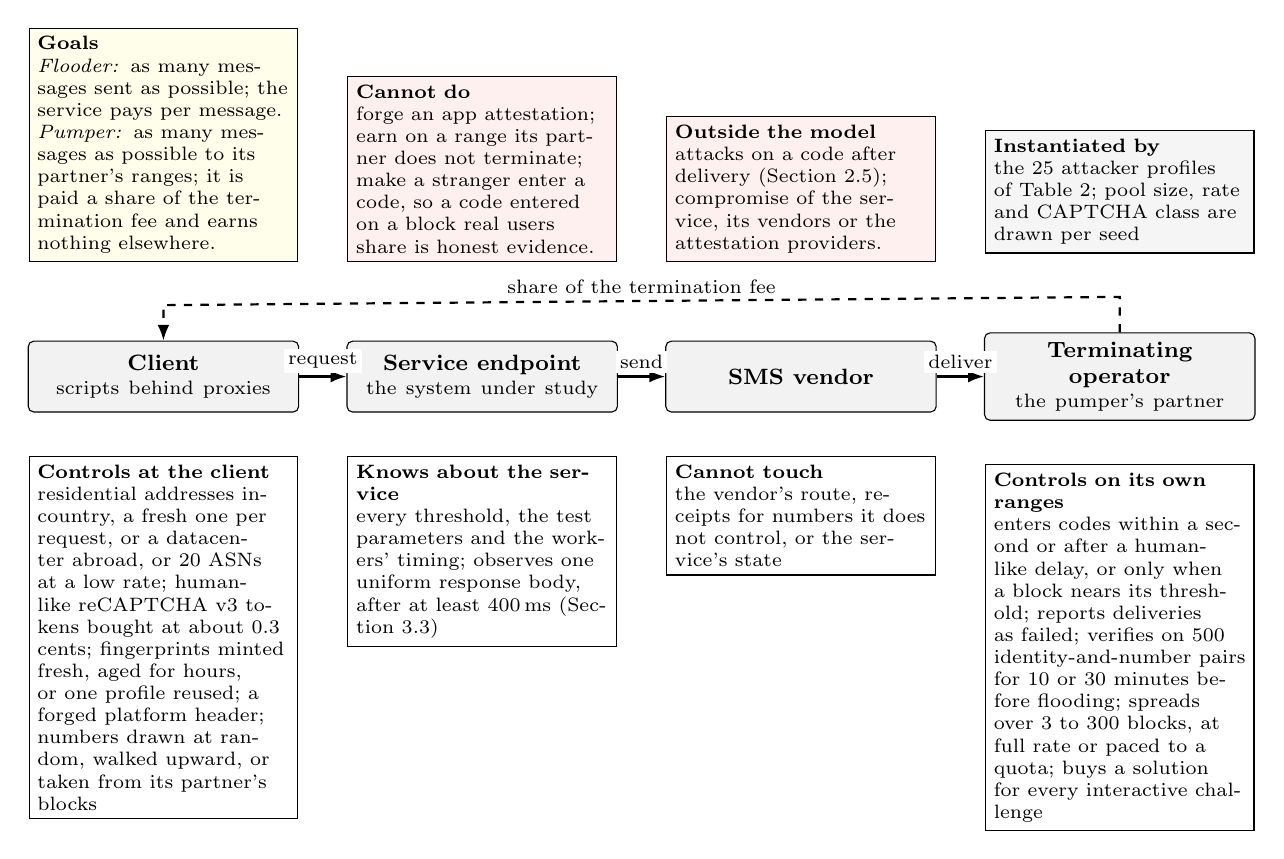
\begin{tikzpicture}[
  stage/.style={draw, rounded corners=2pt, align=center, minimum height=0.9cm, text width=3.2cm, font=\footnotesize\bfseries, fill=gray!10},
  capbox/.style={draw, align=left, text width=3.2cm, font=\scriptsize, inner sep=3pt, fill=white},
  goal/.style={draw, align=left, text width=3.2cm, font=\scriptsize, inner sep=3pt, fill=yellow!8},
  limit/.style={draw, align=left, text width=3.2cm, font=\scriptsize, inner sep=3pt, fill=red!6},
  head/.style={font=\scriptsize\bfseries, anchor=south west},
  arr/.style={-{Latex[length=2mm]}, thick},
  back/.style={-{Latex[length=2mm]}, thick, dashed},
  lab/.style={font=\scriptsize, fill=white, inner sep=1.5pt}
]
% the path
\node[stage] (client) {Client\\[-1pt]{\mdseries\scriptsize scripts behind proxies}};
\node[stage, right=0.6cm of client] (service) {Service endpoint\\[-1pt]{\mdseries\scriptsize the system under study}};
\node[stage, right=0.6cm of service] (vendor) {SMS vendor};
\node[stage, right=0.6cm of vendor] (operator) {Terminating operator\\[-1pt]{\mdseries\scriptsize the pumper's partner}};
\draw[arr] (client) -- node[lab, above=1pt]{request} (service);
\draw[arr] (service) -- node[lab, above=1pt]{send} (vendor);
\draw[arr] (vendor) -- node[lab, above=1pt]{deliver} (operator);
\draw[back] (operator.north) -- ++(0,0.45) -- node[lab, above=1pt]{share of the termination fee} ([yshift=0.45cm]client.north) -- (client.north);

% what the attacker controls, under the points where it acts
\node[capbox, below=0.55cm of client] (cclient) {\textbf{Controls at the client}\\
residential addresses in-country, a fresh one per request, or a datacenter abroad, or 20 ASNs at a low rate; human-like reCAPTCHA v3 tokens bought at about 0.3 cents; fingerprints minted fresh, aged for hours, or one profile reused; a forged platform header; numbers drawn at random, walked upward, or taken from its partner's blocks};
\node[capbox, below=0.55cm of service] (cservice) {\textbf{Knows about the service}\\
every threshold, the test parameters and the workers' timing; observes one uniform response body, after at least 400\,ms (Section 3.3)};
\node[capbox, below=0.55cm of vendor] (cvendor) {\textbf{Cannot touch}\\
the vendor's route, receipts for numbers it does not control, or the service's state};
\node[capbox, below=0.55cm of operator] (coperator) {\textbf{Controls on its own ranges}\\
enters codes within a second or after a human-like delay, or only when a block nears its threshold; reports deliveries as failed; verifies on 500 identity-and-number pairs for 10 or 30 minutes before flooding; spreads over 3 to 300 blocks, at full rate or paced to a quota; buys a solution for every interactive challenge};

% goals and limits, above the path
\node[goal, above=1.0cm of client] (goal) {\textbf{Goals}\\
\emph{Flooder:} as many messages sent as possible; the service pays per message.\\
\emph{Pumper:} as many messages as possible to its partner's ranges; it is paid a share of the termination fee and earns nothing elsewhere.};
\node[limit, above=1.0cm of service] (lim) {\textbf{Cannot do}\\
forge an app attestation; earn on a range its partner does not terminate; make a stranger enter a code, so a code entered on a block real users share is honest evidence.};
\node[limit, above=1.0cm of vendor] (out) {\textbf{Outside the model}\\
attacks on a code after delivery (Section 2.5); compromise of the service, its vendors or the attestation providers.};
\node[capbox, above=1.0cm of operator, fill=gray!8] (prof) {\textbf{Instantiated by}\\
the 25 attacker profiles of Table 2; pool size, rate and CAPTCHA class are drawn per seed};
\end{tikzpicture}
\end{document}
